\section{Equality of Cumulative Votes \label{ecv}}

In the last section we described the execution of the systematic literature review. In order to perform a more thorough analysis later we here present the design of ECV before presenting the results of the systematic literature review. For the results of the evaluation of ECV please see Section~\ref{rq3} (ECV is implemented in the $R$ programming language \citep{Ihaka1996} and the code can be found at \citep{Rinkevics2011}.)

In CV stakeholders may assign similar or equal values to several prioritization items. As a result the difference between the items is small. The variation in priorities is caused not only by the difference between prioritization items but also by human error and lack of information for decision making. For instance, people tend to simplify the task of prioritization by assigning rounded values to items or giving equal values to several items \citep{Groves2009}.

During prioritization it may be beneficial to know which items are equal. A common example is software release planning where requirements are distributed among several product releases. If two or more requirements are considered equal they can be freely interchanged between the releases, and other criteria, such as cost or effort, may be used to used as sole indicators for planning that particular release.

% testing equality
\subsection{\label{Testing-Equality-of}Testing Equality of Two Items}
There are two ways to determine which prioritization items have similar priority.
One approach is to find items that are different and consider other items as equal.
Another approach is to find items that are equal.

The first approach uses statistical tests to evaluate differences between two population means in order to determine that two items are different.
Populations in this case consist of priorities assigned by all stakeholders to a particular prioritization item.
The number of stakeholders that perform the prioritization is frequently small.
Hence, the size of the sample is very often too small for statistical tests to detect a significant difference and the tests, thus, identify too many equal items to make any useful conclusions.

ECV, in contrast, uses the second approach.
It finds items that are similar and the rest of the items are considered different.
This method tests the probability of the difference between the means of two items being smaller than the given value. In short, ECV tests the probability of the means of two prioritization items differing by less than 25\%.
If the probability is higher than 70\% the items are considered equal.

The input to ECV is an $n\times p$ matrix $A$ that contains the raw results of the prioritization.
The columns of the matrix represent prioritization items while rows represent stakeholders.
ECV performs the following operations for the priorities of each two prioritization items:

\begin{enumerate}
\item Replace zeroes in CV results.
\item Transform the data using $ilr$ transformation.
\item Determine distribution function using kernel density estimation.
\item Use the distribution function to find the probability that the difference between two prioritization items is smaller than 25\%.
\item Form groups of equal prioritization items.
\end{enumerate}

Since CV results are compositional data, zeroes in $A$ must be replaced with other values.
This is done using the multiplicative replacement strategy which is described in Section~\ref{Problem-of-Zeroes}.
Next, two columns are extracted from matrix $A$ to create the new matrix $B$:
\begin{equation}
	B=\left[a_{*,k}a_{*,l}\right]\label{eq:b}
\end{equation}
	
where $a$ is an element of matrix $A$, and $k$ and $l$ are the columns that represent items that are tested for equality.

The $ilr$ transformation is then applied to each row of the matrix $B$ and the new vector $C$ is obtained. The equation for calculating elements of $C$ using $ilr$ transformation is:

\begin{equation}
	c_{i}=ilr(b_{i1},b_{i2})=\sqrt{0.5}\log(b_{i1}/b_{i2})\label{eq:c}
\end{equation}

where $c_{i}$ is the $i^{th}$element of $C$ and $b_{i1}$ and $b_{i2}$ are the first and second elements in the $i^{th}$ row of $B$.
Each value $c_{i}$ represents a ratio between $k$ and $l$.
The mean of the values of $C$ can be interpreted as an average ratio between the items that expresses the difference between the items.

After the data is transformed into log-ratios statistical test can be applied.
The purpose of the test is to determine what the probability is of the relative difference between two prioritization items $k$ and $l$ being less than 25\%.
This means determining the probability of the ratio $k/l$ between the items $k$ and $l$ as being in the range of $\frac{3}{4}$ to $\frac{4}{3}$. Or in terms of log-ratios it means determining the probability of $ilr(k,l)$ being between $ilr(3,4)$ and $ilr(4,3)$.
Hence, the objective of the test is to determine the probability of the sample mean (i.e.\ mean value of $C$) laying between the two values.

The probability that the mean takes a particular value can be expressed in form of a cumulative distribution function.
The probability of the mean being between two values $a$ and $b$ (where $a$ is smaller than $b$) can be determined by subtracting the probability of the mean being smaller than $a$ from probability of the mean being smaller than $b$.

However, CV result data may or may not be normally distributed.
If the data is normally distributed a Student's $t$ distribution function can be used.

Otherwise a non-parametric estimation of the distribution function is needed.
In our case, the CV result data obtained from the primary studies identified by the systematic review, were tested for normality using the Anderson-Darling test.
The tests we performed indicated, quite strongly, that in most of the prioritization cases the data is not normally distributed.
Hence, our recommendation is that, in general, a non-parametric approach should be used to determine the probability density function, and one such, common, approach would be to use the kernel density estimation.
(In our implementation of ECV in the $R$ programming language, kernel density estimation is performed using the package $ks$.)

To determine the probability of $\bar{x}$ being between $a$ and $b$ the following equation is used:
\begin{equation}
	p=P(b)-P(a)\label{eq:mean-between-a-b}
\end{equation}

where $P$ is the cumulative distribution function obtained by applying kernel density estimation on $ilr$-transformed priority values denoted by vector $C$. Variable $a$ is equal to $ilr(3,4)$ and $b$ is equal to $ilr(4,3)$. (A graphical interpretation of Equation~(\ref{eq:mean-between-a-b}) is presented in Figure~\ref{fig:Probability-p-that}.)
The area that is denoted by letter $p$ represents the probability computed by the equation.

\begin{figure}
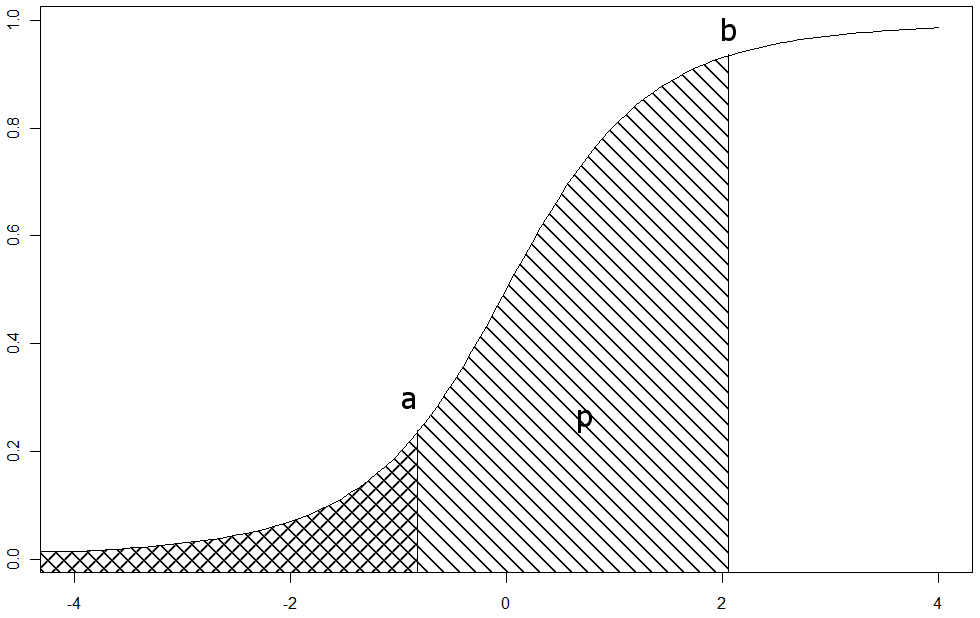
\includegraphics[scale=0.3]{fig/p}
\caption{
	\label{fig:Probability-p-that}
	Cumulative distribution function of 
	the ratio $k/l$ between the items $k$ and $l$
	(area p denotes probability that $k/l$ is between 3/4 and 4/3)
}
\end{figure}

After both prioritization items are tested for equality it may
be convenient to display the equality of different items in the form of a table.
Please see Table~\ref{tab:ECVexample} for an example.

\begin{table}
\caption{Example of equality table}

\label{tab:ECVexample}
\begin{tabular}{|c|c|c|c|c|}
\hline 
prioritization items & i1 & i2 & i3 & i4\tabularnewline
\hline\hline 
i1 & equal & equal & - & equal\tabularnewline
\hline 
i2 & equal & equal & - & -\tabularnewline
\hline 
i3 & - & - & equal & -\tabularnewline
\hline 
i4 & equal & - & - & equal\tabularnewline
\hline
\end{tabular}
\end{table}

\subsection{Grouping Prioritization Items}

When equal items are determined they must be divided into groups of equal items. Division must be performed in such a way that each two items in a group are equal. The test for equality of the items described in Section~\ref{Testing-Equality-of} is not transitive. Hence, if prioritization item $A$ is equal to $B$ and $B$ is equal to $C$ then it does not automatically imply that $A$ is equal to $C$. Therefore, there may be several ways to group the equal items. The two possible division criteria that we have considered in this study are:

\begin{enumerate}
\item Maximize the number of items that have a group.
\item Maximize the number of items in each group.
\end{enumerate}
